%%%%%%%%%%%%%%%%%%%%%%%%%%%%%%%%%%%%%%%%%
% Wenneker Article
% LaTeX Template
% Version 2.0 (28/2/17)
%
% This template was downloaded from:
% http://www.LaTeXTemplates.com
%
% Authors:
% Vel (vel@LaTeXTemplates.com)
% Frits Wenneker
%
% License:
% CC BY-NC-SA 3.0 (http://creativecommons.org/licenses/by-nc-sa/3.0/)
%
%%%%%%%%%%%%%%%%%%%%%%%%%%%%%%%%%%%%%%%%%

%----------------------------------------------------------------------------------------
%	PACKAGES AND OTHER DOCUMENT CONFIGURATIONS
%----------------------------------------------------------------------------------------

\documentclass[12pt, a4paper, twocolumn]{article} % 10pt font size (11 and 12 also possible), A4 paper (letterpaper for US letter) and two column layout (remove for one column)

%%%%%%%%%%%%%%%%%%%%%%%%%%%%%%%%%%%%%%%%%
% Wenneker Article
% Structure Specification File
% Version 1.0 (28/2/17)
%
% This file originates from:
% http://www.LaTeXTemplates.com
%
% Authors:
% Frits Wenneker
% Vel (vel@LaTeXTemplates.com)
%
% License:
% CC BY-NC-SA 3.0 (http://creativecommons.org/licenses/by-nc-sa/3.0/)
%
%%%%%%%%%%%%%%%%%%%%%%%%%%%%%%%%%%%%%%%%%

%----------------------------------------------------------------------------------------
%	PACKAGES AND OTHER DOCUMENT CONFIGURATIONS
%----------------------------------------------------------------------------------------

\usepackage[english]{babel} % English language hyphenation

\usepackage{microtype} % Better typography

\usepackage{amsmath,amsfonts,amsthm} % Math packages for equations

\usepackage[svgnames]{xcolor} % Enabling colors by their 'svgnames'

\usepackage[hang, small, labelfont=bf, up, textfont=it]{caption} % Custom captions under/above tables and figures

\usepackage{booktabs} % Horizontal rules in tables

\usepackage{lastpage} % Used to determine the number of pages in the document (for "Page X of Total")

\usepackage{graphicx} % Required for adding images

\usepackage{enumitem} % Required for customising lists
\setlist{noitemsep} % Remove spacing between bullet/numbered list elements

\usepackage{sectsty} % Enables custom section titles
\allsectionsfont{\usefont{OT1}{phv}{b}{n}} % Change the font of all section commands (Helvetica)

%----------------------------------------------------------------------------------------
%	MARGINS AND SPACING
%----------------------------------------------------------------------------------------

\usepackage{geometry} % Required for adjusting page dimensions

\geometry{
	top=2cm, % Top margin
	bottom=2.5cm, % Bottom margin
	left=2cm, % Left margin
	right=2cm, % Right margin
	includehead, % Include space for a header
	includefoot, % Include space for a footer
	%showframe, % Uncomment to show how the type block is set on the page
}

\setlength{\columnsep}{8mm} % Column separation width

%----------------------------------------------------------------------------------------
%	FONTS
%----------------------------------------------------------------------------------------

\usepackage[T1]{fontenc} % Output font encoding for international characters
\usepackage[utf8]{inputenc} % Required for inputting international characters

\usepackage{XCharter} % Use the XCharter font
\usepackage{float}
%----------------------------------------------------------------------------------------
%	HEADERS AND FOOTERS
%----------------------------------------------------------------------------------------

\usepackage{fancyhdr} % Needed to define custom headers/footers
\pagestyle{fancy} % Enables the custom headers/footers

\renewcommand{\headrulewidth}{0.0pt} % No header rule
\renewcommand{\footrulewidth}{0.4pt} % Thin footer rule

\renewcommand{\sectionmark}[1]{\markboth{#1}{}} % Removes the section number from the header when \leftmark is used

%\nouppercase\leftmark % Add this to one of the lines below if you want a section title in the header/footer

% Headers
\lhead{} % Left header
\chead{\textit{\thetitle}} % Center header - currently printing the article title
\rhead{} % Right header

% Footers
\lfoot{} % Left footer
\cfoot{} % Center footer
\rfoot{\footnotesize Page \thepage\ of \pageref{LastPage}} % Right footer, "Page 1 of 2"

\fancypagestyle{firstpage}{ % Page style for the first page with the title
	\fancyhf{}
	\renewcommand{\footrulewidth}{0pt} % Suppress footer rule
}

%----------------------------------------------------------------------------------------
%	TITLE SECTION
%----------------------------------------------------------------------------------------

\newcommand{\authorstyle}[1]{{\large\usefont{OT1}{phv}{b}{n}\color{DarkRed}#1}} % Authors style (Helvetica)

\newcommand{\institution}[1]{{\footnotesize\usefont{OT1}{phv}{m}{sl}\color{Black}#1}} % Institutions style (Helvetica)

\usepackage{titling} % Allows custom title configuration

\newcommand{\HorRule}{\color{DarkGoldenrod}\rule{\linewidth}{1pt}} % Defines the gold horizontal rule around the title

\pretitle{
	\vspace{-30pt} % Move the entire title section up
	\HorRule\vspace{10pt} % Horizontal rule before the title
	\fontsize{32}{36}\usefont{OT1}{phv}{b}{n}\selectfont % Helvetica
	\color{DarkRed} % Text colour for the title and author(s)
}

\posttitle{\par\vskip 15pt} % Whitespace under the title

\preauthor{} % Anything that will appear before \author is printed

\postauthor{ % Anything that will appear after \author is printed
	\vspace{10pt} % Space before the rule
	\par\HorRule % Horizontal rule after the title
	\vspace{25pt} % Space after the title section
}

%----------------------------------------------------------------------------------------
%	ABSTRACT
%----------------------------------------------------------------------------------------

\usepackage{lettrine} % Package to accentuate the first letter of the text (lettrine)
\usepackage{fix-cm}	% Fixes the height of the lettrine

\newcommand{\initial}[1]{ % Defines the command and style for the lettrine
	\lettrine[lines=3,findent=4pt,nindent=0pt]{% Lettrine takes up 3 lines, the text to the right of it is indented 4pt and further indenting of lines 2+ is stopped
		\color{DarkGoldenrod}% Lettrine colour
		{#1}% The letter
	}{}%
}

\usepackage{xstring} % Required for string manipulation

\newcommand{\lettrineabstract}[1]{
	\StrLeft{#1}{1}[\firstletter] % Capture the first letter of the abstract for the lettrine
	\initial{\firstletter}\textbf{\StrGobbleLeft{#1}{1}} % Print the abstract with the first letter as a lettrine and the rest in bold
}

%----------------------------------------------------------------------------------------
%	BIBLIOGRAPHY
%----------------------------------------------------------------------------------------

\usepackage[backend=bibtex,style=authoryear,natbib=true]{biblatex} % Use the bibtex backend with the authoryear citation style (which resembles APA)

\addbibresource{example.bib} % The filename of the bibliography

\usepackage[autostyle=true]{csquotes} % Required to generate language-dependent quotes in the bibliography
 % Specifies the document structure and loads requires packages

%----------------------------------------------------------------------------------------
%	ARTICLE INFORMATION
%----------------------------------------------------------------------------------------

\title{A Comparative Study of DQN Performance in Atari Pong with Varying Environment Frame Rates} % The article title

\author{
	\authorstyle{James Bardin \textsuperscript{1}} % Authors
	\newline\newline % Space before institutions
	\textsuperscript{1}\institution{Harvard University, Cambridge, Massachusetts}\\ % Institution 1
}

% Example of a one line author/institution relationship
%\author{\newauthor{John Marston} \newinstitution{Universidad Nacional Autónoma de México, Mexico City, Mexico}}

\date{\today} % Add a date here if you would like one to appear underneath the title block, use \today for the current date, leave empty for no date

%----------------------------------------------------------------------------------------

\begin{document}

\maketitle % Print the title

\thispagestyle{firstpage} % Apply the page style for the first page (no headers and footers)

%----------------------------------------------------------------------------------------
%	ABSTRACT
%----------------------------------------------------------------------------------------

\lettrineabstract{Question: Can Deep Q-Networks (DQN) trained on Pong Environments with specific frame rates generalize to perform well on environments with different frame rates, and, are different training frame rates better at generalizing?}

%----------------------------------------------------------------------------------------
%	ARTICLE CONTENTS
%----------------------------------------------------------------------------------------

\section{Literature Review}

Over the last decade there has been tremendous progress in the field of deep reinforcement learning, which has led to breakthroughs in industry automation, healthcare, natural language processesing, and even gaming. With no prior knowledge, reinforment learning agents are able to learn and master video game control strategies in times that humans don't come close to matching. One of the leading works in this area, cited over ten thousand times, is the paper "Playing Atari with Deep Reinforcement Learning" by Mnih et al. (2013). The authors demonstrated the effectiveness of a DQN algorithm in playing classic Atari games, achieving superhuman performance on several different games without any adjustments to architecture or learning algorithm.

Since then, various modifications and extensions to the DQN algorithm have been proposed to improve its performance and stability. Deep reinforcement learning has significant challenge with computational requirements. The complexity of the algorithms are tough to reduce because of the inherent requirement for sequentiality. Training data is generated during learning which seemingly leaves few options for significant speed and computational improvements. But, in ”Reinforcement learning through asynchronous advantage actor-critic on a GPU” by Mnih et al. (2016) exmplores different possibilities. The main issue is that training batches are typically small and need to be efficiently guided to the DNN trainer. And, when using a GPU, small DNN architectures, small batches, both lead to sub-optimal utilization of computational resources. One modification they proposed was the asynchronous advantage actor-critic (A3C) algorithm, which enables parallel learning on a GPU and was found to achieve state-of-the-art results on several benchmark tasks.

More recently, the paper "Human-level control through deep reinforcement learning" also by Mnih et al. (2015) explored the potential that deep reinforcement learning algorithms have in solving more complex tasks, such as controlling a simulated humanoid robot, or again playing many different Atari 2600 games. The authors used a variant of the DQN algorithm called deep reinforcement learning with double Q-learning (DDQN) algorithm. And, they found they could acheive better performance and stability compared to the original DQN algorithm.

Each one of these papers highlight the leaps and bounds made in the field of deep reinforcement learning, as well as the potential these algorithms have to solve complex tasks, yet, reinforcement learning is a still blossoming field with countless discoveries and improvemnts left to be made. Some areas being focused on by research groups around the world include improving the sample efficiency, scalability, and generalizability of these algorithms to tasks that stray from the training situation.

%------------------------------------------------

\section{Methodology}

\subsection{Experience Replay}
The implementation contains several main components that work together to traing an agent to solve Atari pong. First, we have our experience replay. The pseudocode for this section is as follows:

\begin{figure}[H]
	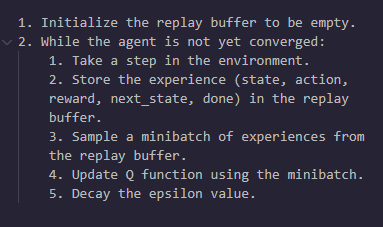
\includegraphics[width=\linewidth]{experience_replay_pseudocode.PNG} % Figure image
\end{figure}

The experience buffer is a data structure that is used to maintain a history of past experiences. The experience buffer is accessed by the agent to store experiences as it takes steps through the environment. An experience, as shown in the pseudocode, contains the state, the action the agent took, the reward as a result of the action, the next state the agent is then in, and a boolean indicating whether the game has ended or not. The agent then takes a minibatch (a small subset) of experiences that are stored in the experience buffer using the defined experience data type, and uses these to update the Q-function with a method known as back propogation. The epsilon value we see in part 2-5 is another key concept. The epsilon is a hyperparameter that was carefully adjusted because it is responsible for controling the exploration-exploitation trade off. When there is a high epsilon value, there are higher odds that the agent will make decisions--that according to what the agent knows--are suboptimal. And it does this with hopes of escaping local extrema because when the agent is still young (hasn't observed significant data), it is likely to think that suboptimal strategies are optimal. So, as the epsilon decays, it takes fewer and fewer risky moves, more often sticking to what it has learned to work well. The experience buffer is implemented here \textbf{INSERT LINK HERE}. 

\subsection{Agent Class}

Next the agent class was implemented. The agent class is used to determine the actions the agent takes inside of the environment we place it in. The agent class takes two parameters in its' constructor: the environment and the experience buffer. It contains several methods such as reset, which puts the agent's state back to the start and resets the total reward, used at the beginning of each game. It also has a play step function that takes an action according to the epsilon-greedy policy. The play step function takes a neural network, epsilon, and device as parameters. The neural network is what is used to estimate the Q-values of an action. The epsilon, determines the probiability that the agent takes a risk step vs an well informed step. A random number is generated from 0 to 1 and if the epsilon is less than the number it chooses the action with the highest estimated Q-value from the neural network, and if it is less than the epsilon it will take a random action from the environment's action space. And finally, the device is where the neural network is being run on, so the CPU or the GPU. The agent class is implemented here \textbf{INSERT LINK HERE}. 

\subsection{Loss Function}

Then, we have the implementation of the loss function. The loss function uses mean squeared error (from torch.nn) to calculate loss. the function takes in a batch of data, the neural network, the target network and the device. The batch of data, containing the same as the batches described before (state, actions, ...) are converted to PyTorch tensors and moved to the device for computation. The neural network is used to predict the Q-values for the state-action pairs. And the returned Q-value we treat as the expected sum of future rewards based on the action that was taken in the current state. Next, the target network is used to estimate the Q-value again, but now of the next state that has the highest Q-value. And this value is used to calculate the expected Q-value for the state-action pair by summing the immediate reward and future rewards. And finally, the expected Q-value is compared with the predicted from the mean square error function and returned. The loss function is implemented here \textbf{INSERT LINK HERE}. 

\subsection{Environment}

The environment used for training is created from OpenAI's gym library. OpenAI has public wrappers for environments that make training an agent much easier. Examples of the wrappers implemented will start environments by pressing fire, apply various image preprocessing techniques such as data conversions, cropping, pixel reduction, and most importatnly for this project, reduce the number of frames that are taken from the environment. We modified some parts of the wrappers from OpenAI and implemented the changes here \textbf{INSERT LINK HERE} in a file called wrappers skips. 

\subsection{Neural Networks}

Then, the neural networks were implemented using the DQN class defined in the file named dqn model, which is a subclass of the torch.nn.Module class from PyTorch. The model is a standard, simplified version of the model described in "Human-level control through deep reinforcement learning". It consists of a 4 layer CNN to extract features from the game state. And a fully connected network to predict Q-values for each action. The model is trained using a Q-learning algorithm, which updates Q-values for each state-action pair $(s,a)$,

\[  Q(s,a) \leftarrow Q(s,a) + \alpha (r + \gamma \max_{a'} Q(s',a') - Q(s,a))  \]

Where alpha is the learning rate, $r$ is the reward for some action $a$ taken in a state $s$. The primes indicate the next state, and gamma is the discount factor. The DQN is trained using the experience buffer, which improves stability by preventing overfitting to training data. And, after training on a parameter grid, we found the most success using Adam's optimizer to optimize the network parameters. 

\subsection{Main Training Loop}

So, that remains the is implementation the main training loop for the network. The network is trained by both using the experience buffer and the loss fuction. The target network is periodically updated (promoting stability). And, this training continues until the mean reward exceeds some predefined bound at which we consider the environment solved, or until is reaches a predefined number of games. The main loop follows the following pseudocode,

\begin{figure}[H]
	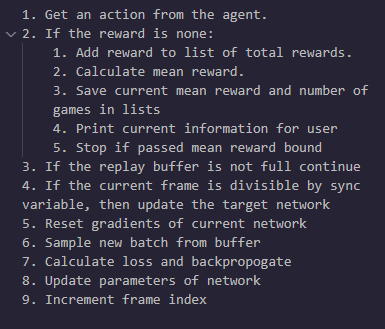
\includegraphics[width=\linewidth]{traing_loop_pseudocode.PNG} % Figure image
\end{figure}


%------------------------------------------------

\subsection{Conda Environment}

This program was implemented inside a Conda environment with python 3.9.13. A yaml is provided in the Git repository called tfgpu env. This environment was designed for GPU acceleration support for Windows 10 with the help of Bex T.'s article published on Towards Data Science titled "How to Finally Install TensorFlow 2 GPU on Windows 10".


%------------------------------------------------

\section{Results}

Due to time constraints, many of the frame skip rates we only ran until we began to see significant decay in mean reward improvement rate, for somewhere around six hours on average. But, for five different frame rate values (skip every 3rd, 4th, 5th and 9th frames), we let the agent train for over 12 hours each. And, as a result we have well developed and highly performing agents in each of the environment types, and especially well performing models in the give environment types that were just specified. The plots for all skip rates from three to nine are shown below.


\begin{figure}[H]
	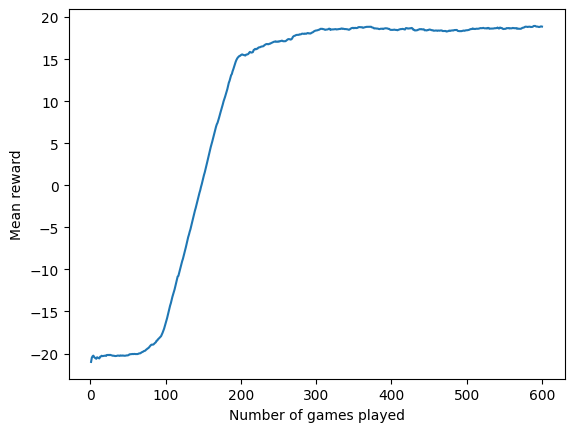
\includegraphics[width=\linewidth]{mr_sk3.PNG} % Figure image
	\caption{Mean Reward: Skip Every 3rd Frame} % Figure caption
\end{figure}

\begin{figure}[H]
	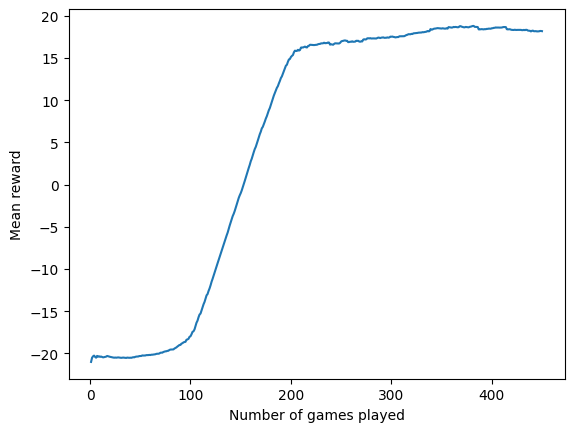
\includegraphics[width=\linewidth]{mr_sk4.PNG} % Figure image
	\caption{Mean Reward: Skip Every 4th Frame} % Figure caption
\end{figure}

\begin{figure}[H]
	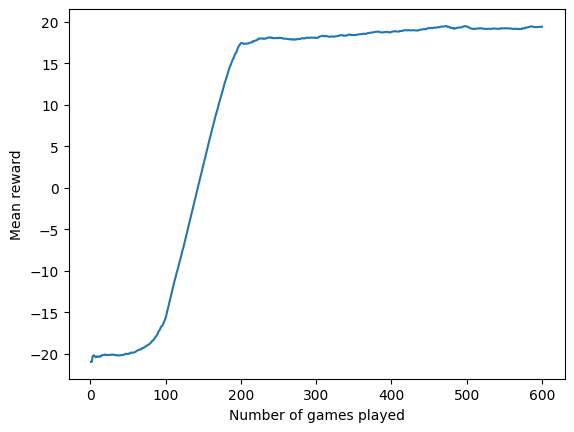
\includegraphics[width=\linewidth]{mr_sk5.PNG} % Figure image
	\caption{Mean Reward: Skip Every 5th Frame} % Figure caption
\end{figure}

\begin{figure}[H]
	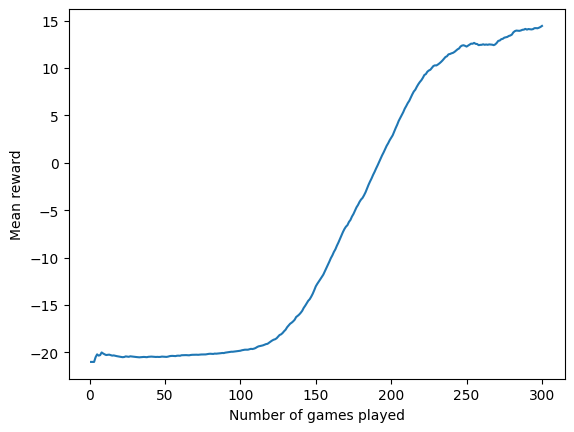
\includegraphics[width=\linewidth]{mr_sk6.PNG} % Figure image
	\caption{Mean Reward: Skip Every 6th Frame} % Figure caption
\end{figure}

\begin{figure}[H]
	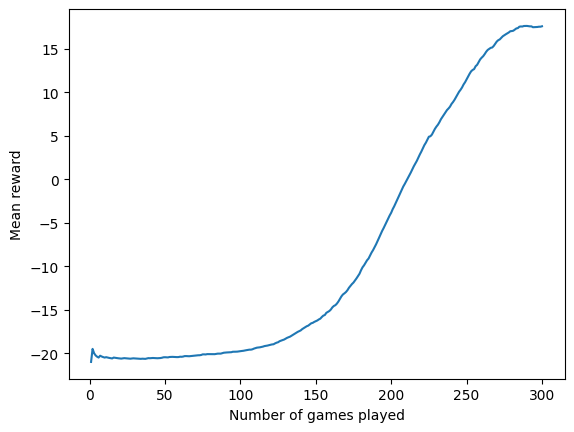
\includegraphics[width=\linewidth]{mr_sk7.PNG} % Figure image
	\caption{Mean Reward: Skip Every 7th Frame} % Figure caption
\end{figure}

\begin{figure}[H]
	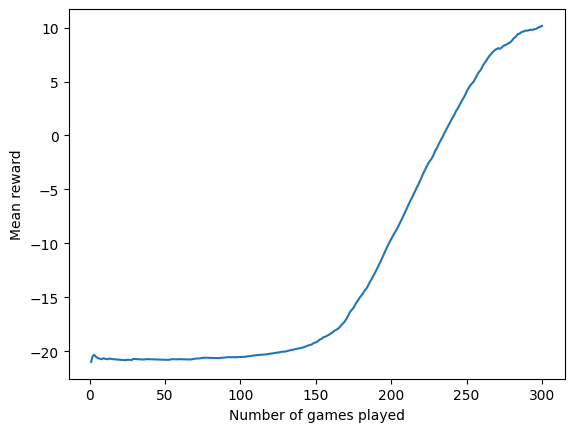
\includegraphics[width=\linewidth]{mr_sk8.PNG} % Figure image
	\caption{Mean Reward: Skip Every 8th Frame} % Figure caption
\end{figure}

\begin{figure}[H]
	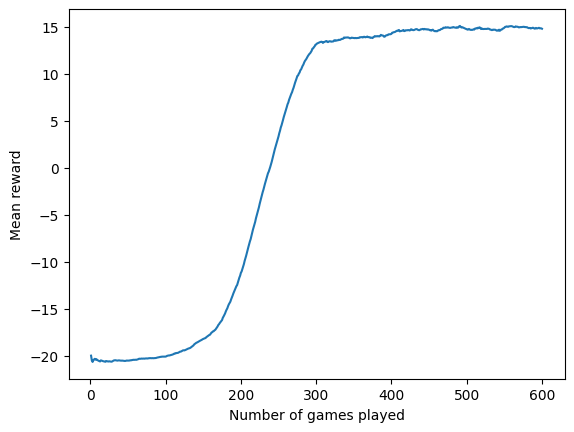
\includegraphics[width=\linewidth]{mr_sk9.PNG} % Figure image
	\caption{Mean Reward: Skip Every 9th Frame} % Figure caption
\end{figure}



\begin{figure}[H]
	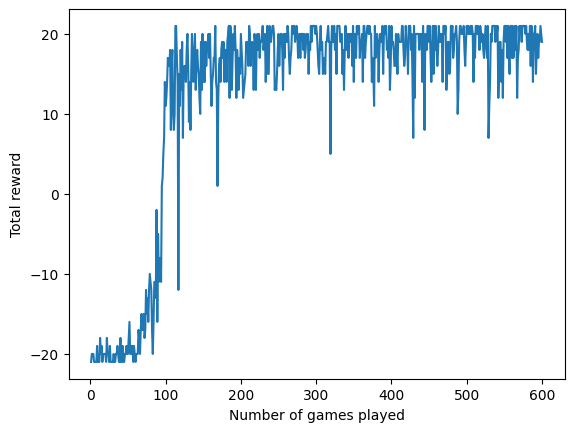
\includegraphics[width=\linewidth]{tr_sk3.PNG} % Figure image
	\caption{Total Reward: Skip Every 3rd Frame} % Figure caption
\end{figure}

\begin{figure}[H]
	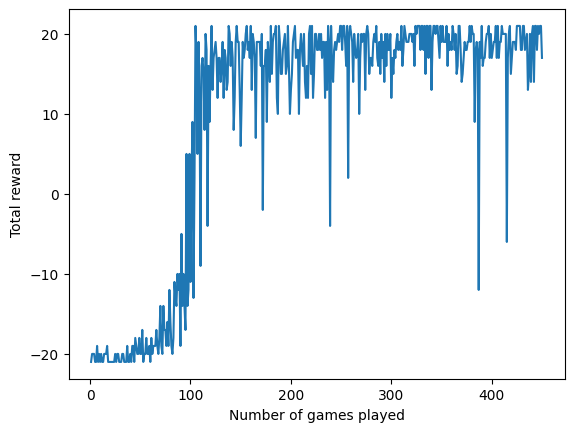
\includegraphics[width=\linewidth]{tr_sk4.PNG} % Figure image
	\caption{Total Reward: Skip Every 4th Frame} % Figure caption
\end{figure}

\begin{figure}[H]
	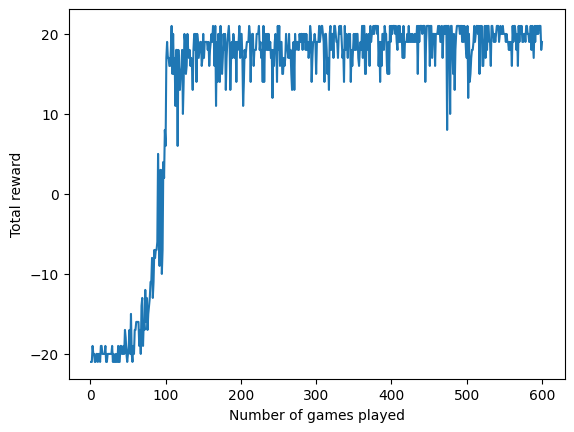
\includegraphics[width=\linewidth]{tr_sk5.PNG} % Figure image
	\caption{Total Reward: Skip Every 5th Frame} % Figure caption
\end{figure}

\begin{figure}[H]
	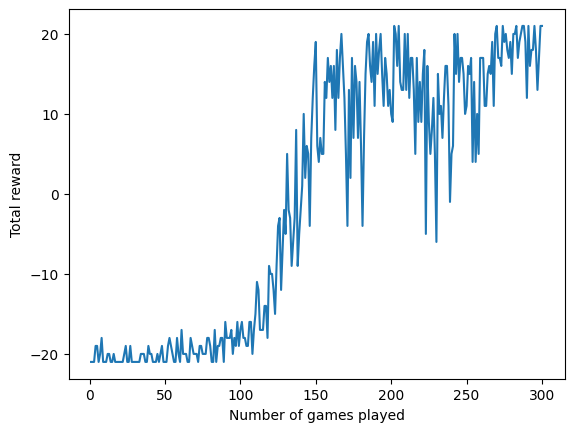
\includegraphics[width=\linewidth]{tr_sk6.PNG} % Figure image
	\caption{Total Reward: Skip Every 6th Frame} % Figure caption
\end{figure}

\begin{figure}[H]
	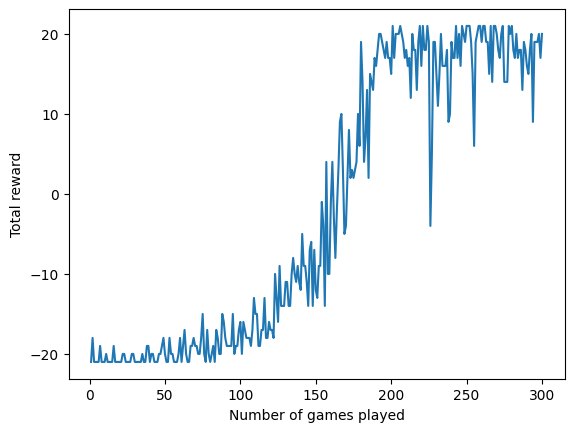
\includegraphics[width=\linewidth]{tr_sk7.PNG} % Figure image
	\caption{Total Reward: Skip Every 7th Frame} % Figure caption
\end{figure}

\begin{figure}[H]
	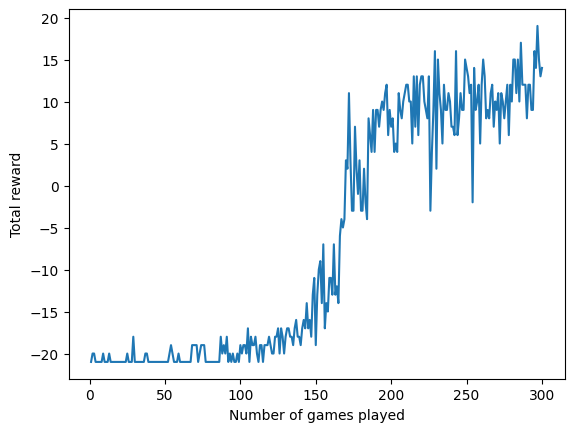
\includegraphics[width=\linewidth]{tr_sk8.PNG} % Figure image
	\caption{Total Reward: Skip Every 8th Frame} % Figure caption
\end{figure}

\begin{figure}[H]
	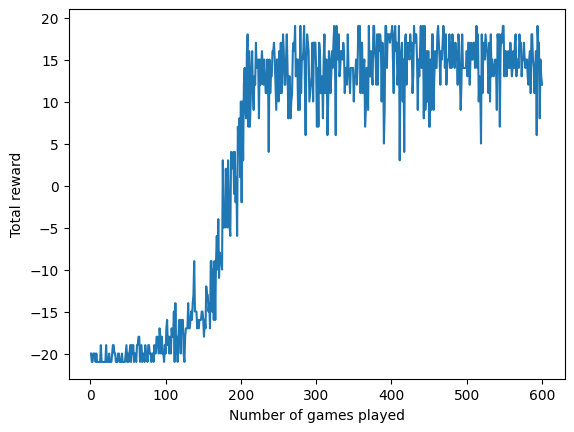
\includegraphics[width=\linewidth]{tr_sk9.PNG} % Figure image
	\caption{Total Reward: Skip Every 9th Frame} % Figure caption
\end{figure}

\subsection{Further Examination and Dicussion}

After we had trained all of these models, until they were consistently beating the opponent handidly, we examined the generalizability to different environment frame rates. We ran agents trained by models with frame skip rate of 3, 5, 7, and 9, on environments with values of frame skip rates within an integer value 2 from the rate. Each frame skip rate was run on each environment 20 times, and the average rewards were saved and plotted. We got the following,

\begin{figure}[H]
	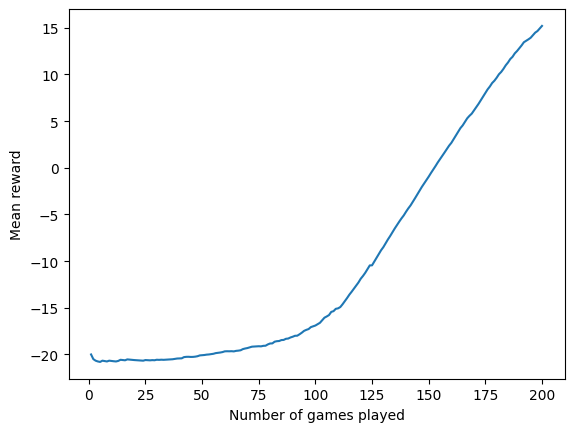
\includegraphics[width=\linewidth]{output.PNG} % Figure image
	\caption{Performance on Varying Framerates} % Figure caption
\end{figure}

Interestingly, the models were very poor at performing in environments with frame rates different from the environment they were tested in. When I first noticed this, I was curious if there was any performance improvements in models that skipped the same or different polarity frames, or where the frame skip was a multiple of the other one. For instance, would an environment that checks every third frame perform well in an environment checks every sixth frame or vice versa, and it turned out that none of these very able to generalize to other frame rates. This was interesting because it showed how important consistency in preprocessing is to model performance. The agents are trained on environments with specific game rates and thus learned to make decisions based on specific timings and speed of visual cues. Although there is not a perfectly clear explanation for this, one possibility is that when the agent is trained on a very high frame rate, the motion of the ball may not be perceived as linear. Because of the fairly small pixel space, the ball cannot move in a true straight line if it is moving at an angle different than 0, -45, or 45 (if zero is perpendicular to the paddle). In these cases the ball's path would be stepping like a staircase. And, in the case where the agent is trained on a lower frame rate, there is more information losss. And, when in a different environment, the agent would have more trouble accurately perceiving the state of the game. 

Upon this discovery, the question was raised whether the trained agent could adapt to varying initial seeds, since all environments were initialized with the same seed during training. The results showed that even when the environment seeding was randomized, the agent was capable of outperforming the opponent with the same average reward. And, interestingly the agent although begining with a different sequence of volleys, would end up using the same strategy. After winning a point and the ball being served to the opponent, the agent uses the same strategy of bouncing a unreturnable ball off the floor or ceiling (depending on what is closest), always scoring after a single contact when the opponent is served. And interestingly, no matter what frame rate the agent was trained in, it always developed a similar strategy at playing the game. 



%----------------------------------------------------------------------------------------
%	BIBLIOGRAPHY
%----------------------------------------------------------------------------------------

\printbibliography[title={Bibliography}] % Print the bibliography, section title in curly brackets

%----------------------------------------------------------------------------------------

\end{document}
